\appendix
%% Правка оформления ссылок на приложения:
%http://tex.stackexchange.com/questions/56839/chaptername-is-used-even-for-appendix-chapters-in-toc
%http://tex.stackexchange.com/questions/59349/table-of-contents-with-chapter-and-appendix
%% требует двойной компиляции
\addtocontents{toc}{\def\protect\cftchappresnum{\appendixname{} }%
\setlength{\cftchapnumwidth}{\widthof{\cftchapfont\appendixname~Ш\cftchapaftersnum}}%
}
%% Оформление заголовков приложений ближе к ГОСТ:
\sectionformat{\chapter}[display]{% Параметры заголовков разделов в тексте
    label=\chaptertitlename\ \thechapter,% (ГОСТ Р 2.105, 4.3.6)
    labelsep=20pt,
}
\renewcommand\thechapter{\Asbuk{chapter}} % Чтобы приложения русскими буквами нумеровались



\chapter{Структура данных измерений ДЭПРОН} \label{AppendixA}




\section{Блок данных ДЭПРОН A}
\small
\begin{center}	
\begin{tabularx}{\textwidth}{|c|c|c|c| *5{>{\centering\arraybackslash}X|}}
	\hline
	\multicolumn{8}{|c|}{Данные}                                                                                                &  \\
	\multicolumn{8}{|c|}{(RECORD)}                                                                                              &  \\ \hline
	\multicolumn{4}{|c|}{Время }      & Аппаратный счетчик  детектора1 & Счет детектора 1 & Счет детектора 2 & Счет детектора 2 &  \\ \cline{1-4}
	месяц  &  день  &  час   &  мин   &                                &                  &                  &  \\ \hline
	1 байт & 1 байт & 1 байт & 1 байт & 2 байта                        & 2 байта          & 2 байта          & 2 байта          &  \\ \hline
\end{tabularx} 
\end{center}
\normalsize
Продолжение:
\small
\begin{center}	
	\begin{tabularx}{\textwidth}{|*6{>{\centering\arraybackslash}X|}}
		\hline
		\multicolumn{6}{|c|}{Данные}                                                                                                                          \\
		\multicolumn{6}{|c|}{(RECORD)}                                                                                                                        
		\\ \hline
		Нейтронный счетчик 1 & Нейтронный счетчик 	2 & Доза по первому детектору & Доза по второму детектору & Доза совпадений & Массивы секундной динамики 2 
		\\ \hline
		2 байта              & 2 байта               & 4 байта                   & 4 байта                   & 4 байта         & 480 байт                     
		\\ \hline
	\end{tabularx} 
\end{center}
\normalsize



Блок массивов секундной динамики содержат шестьдесят массивов, содержащих приращения значений счетчиков за секунду, сжатых алгоритмом логарифмического сжатия, разработанным В.В. Бенгиным.

\small
\begin{center}	
	\begin{tabularx}{\textwidth}{| *4{>{\centering\arraybackslash}X|}}
		\hline
		\multicolumn{4}{|c|}{Массив секундной динамики}                                           \\ \hline
		Аппаратный счетчик детектора 1 & Счет детектора  1 & Счет детектора 2 & Счет совпадений 1 \\ \hline
		1 байт                         & 1 байт            & 1 байт           & 1 байт            \\ \hline
	\end{tabularx} 
\end{center}
\normalsize
Продолжение:
\small
\begin{center}	
	\begin{tabularx}{\textwidth}{| *4{>{\centering\arraybackslash}X|}}
		\hline
		\multicolumn{4}{|c|}{Массив секундной динамики}                                                     \\ \hline
		Нейтронный счетчик 1 & Нейтронный счетчик 2 & Доза по первому детектору & Доза по второму детектору \\ \hline
		1 байт               & 1 байт               & 1 байт                    & 1 байт                    \\ \hline
	\end{tabularx} 
\end{center}
\normalsize








\section{Блок данных ДЭПРОН S}

\footnotesize
\begin{center}	
	\begin{tabularx}{\textwidth}{|X|c|c|c| *6{>{\centering\arraybackslash}X|}}
		\hline
		\multicolumn{10}{|c|}{Данные}                                                                                                                           
		              \\
		\multicolumn{10}{|c|}{(RECORD)}                                                                                                                         
		              \\ \hline
		Спектр детектора 1 & \multicolumn{4}{|c|}{Время }         & Спектр детектора 2 & Счетчик детектора 1 & Спектр совпадений 1 & Счетчик детектора 2 & 
		Спектр совпадений2 \\ \cline{2-5}
		                   & месяц  &  день  &  час   & мин       &                    &                     &                     &                     &  \\ 
		                   \hline
		124 байта          & 1 байт & 1 байт & 1 байт & 124 байта & 4 байта            & 124 байта           & 4 байта             & 124 байта           & 4 
		байта            \\ \hline
	\end{tabularx} 
\end{center}
\normalsize

Вместо длины сообщения LEN для данного массива в заголовок записывается номер массива спектров (0-255).

Каждый передаваемый спектр содержит число зарегистрированных импульсов, попадающих в соответствующий энергетический канал детектора. Количество энергетических диапазонов 62, верхние границы каналов выбраны с помощью алгоритма логарифмического преобразования номера канала. 

\small
\begin{center}
\begin{tabular}{|*4{|cc|}}
	\hline
	Канал № & Код АЦП & Канал № & Код АЦП & Канал № & Код АЦП & Канал № & Код АЦП \\ \hline
	   2    &   16    &   18    &   160   &   34    &   640   &   50    &  2560   \\ \hline
	   3    &   24    &   19    &   176   &   35    &   704   &   51    &  2816   \\ \hline
	   4    &   32    &   20    &   192   &   36    &   768   &   52    &  3072   \\ \hline
	   5    &   40    &   21    &   208   &   37    &   832   &   53    &  3328   \\ \hline
	   6    &   48    &   22    &   224   &   38    &   896   &   54    &  3584   \\ \hline
	   7    &   56    &   23    &   240   &   39    &   960   &   55    &  3840   \\ \hline
	   8    &   64    &   24    &   256   &   40    &  1024   &   56    &  4096   \\ \hline
	   9    &   72    &   25    &   288   &   41    &  1152   &   57    &  4608   \\ \hline
	  10    &   80    &   26    &   320   &   42    &  1280   &   58    &  5120   \\ \hline
	  11    &   88    &   27    &   352   &   43    &  1408   &   59    &  5632   \\ \hline
	  12    &   96    &   28    &   384   &   44    &  1536   &   60    &  6144   \\ \hline
	  13    &   104   &   29    &   416   &   45    &  1664   &   61    &  6656   \\ \hline
	  14    &   112   &   30    &   448   &   46    &  1792   &   62    &  7168   \\ \hline
	  15    &   120   &   31    &   480   &   47    &  1920   &   63    &  7680   \\ \hline
	  16    &   128   &   32    &   512   &   48    &  2048   &         &  \\ \hline
	  17    &   144   &   33    &   576   &   49    &  2304   &         &  \\ \hline
\end{tabular}  
\end{center}
\normalsize

Таким образом, массивы спектров состоят из 62 четырехбайтных целых значений, порядок которых соответствует приведенному набору каналов.

\section{Блок данных ДЭПРОН H}


\small
\begin{center}
	\begin{tabularx}{\textwidth}{|c|c|X|X|}
		\hline
		\multicolumn{4}{|c|}{Данные (RECORD)}                                                                                          \\ \hline
		\multicolumn{2}{|c|}{Время} & Индекс массива высоких амплитуд(по умолчанию значение 63) & Массивы данных по высоким амплитудам \\ \cline{1-2}
		месяц  &        день        &                                                           &  \\ \hline
		1 байт &       1 байт       & 2 байта                                                   & 63 массива  по 8 байт                \\ \hline
	\end{tabularx}  
\end{center}
\normalsize
	



Структура записи в массивы данных по высоким амплитудам:

\small
\begin{center}
	\begin{tabularx}{\textwidth}{|c|c|X|X|X|X|}
		\hline
		\multicolumn{6}{|c|}{Массив данных по высоким амплитудам}       \\ \hline
		Код АЦП 1 & Код АЦП 2 &   \multicolumn{4}{c|}{Время события}    \\ \cline{3-6}
		          &           & Код таймера & секунда & минута & час    \\ \hline
		 2 байта  &  2 байта  & 1 байт      & 1 байт  & 1 байт & 1 байт \\ \hline
	\end{tabularx}  
\end{center}
\normalsize




\section{Блок данных ДЭПРОН N}

Информация по зарегистрированным нейтронным всплескам представлена в виде блока данных, состоящего из 127 массивов  по 4 байта каждый.
Структура записи в массив данных по нейтронным всплескам :

\small
\begin{flushleft}
	\begin{tabular}{|*{17}{p{0.5cm}|}}
		\hline
		32 & 31 & 30 & 29 & 28 & 27 & 26 & 25 & 24 & 23 & 22 & 21 & 20 & 19 & 18 & 17 & 16 \\ \hline
		\multicolumn{17}{|c|}{Время дня в секундах}                                        \\ \hline
	\end{tabular}  
\end{flushleft}
\normalsize

\small
\begin{flushleft}
	\begin{tabular}{|*{15}{p{0.5cm}|}}
		\hline
		15 & 14                  & 13 & 12 & 11 & 10 & 9 & 8 & 7 & 6 & 5 & 4 & 3 & 2 & 1                                      \\ \hline
		\multicolumn{2}{|c|}{НД} & \multicolumn{13}{p{9cm}|}{Количество тиков таймера после предыдущего нейтронного импульса} \\ \hline
	\end{tabular}  
\end{flushleft}
\normalsize



	НД -- номер сработавшего нейтронного детектора:

	01 -- срабатывание первого детектора

	10 -- срабатывание второго детектора

	11 -- срабатывание обоих детекторов





\section{Блок данных ДЭПРОН Т}

В общей структуре сообщения для данного блока данных не выдается длина сообщения \texttt{LEN}, вместо этого передается {`}\ensuremath{\backslash}0'.(Исправлено 27.02.2013)


Данный блок данных генерируется в ответ на пришедшее по каналу CAN от БИ командное сообщение, либо по мере заполнения выходного буфера при работе в режиме отладки прибора ДЭПРОН.



\section{Команды прибора ДЭПРОН}



Для управления работой прибора ДЭПРОН предусмотрено 6 типов команд:

\begin{itemize}
	\item 	Сброс настроек к заводским параметрам

	\item Увеличение временного диапазона для нейтронных последовательностей

	\item Уменьшение временного диапазона для нейтронных последовательностей

	\item Увеличение полосы фильтра шумов протонных каналов

	\item Уменьшение полосы фильтра шумов протонных каналов

	\item Увеличение интервала времени сглаживания

\end{itemize}


\small
\begin{center}
	\begin{tabularx}{\textwidth}{|c|c|X|}
		\hline
		№ & Команда & Описание команды                                           \\ \hline
		1 &   Clr   & сброс настроек к заводским параметрам                      \\ \hline
		2 &   Tn+   & увеличение интервала между моментами регистрации нейтронов \\ \hline
		3 &   Tn-   & уменьшение интервала между моментами регистрации нейтронов \\ \hline
		4 &  Psnr+  & увеличение допустимого протонного фона                     \\ \hline
		5 & Psnr\_  & уменьшение допустимого протонного фона                     \\ \hline
		6 & Alpha+  & увеличение интервала времени сглаживания                   \\ \hline
	\end{tabularx}  
\end{center}
\normalsize



Ответный массив информации от прибора ДЭПРОН.
\footnotesize
\begin{center}
	\begin{tabularx}{\textwidth}{|*5{c|}|*6{X|}}
		\hline
		\multicolumn{11}{|c|}{Данные 
		(RECORD)}                                                                                                                            \\ \hline
		\multicolumn{5}{|c|}{Время}                & Номер команды породившей ответ & D tick  & Счетчик принятых команд & Текущий фон потока протонов & Psnr    
		& Alfa    \\ \cline{1-5}
		 мес   &  день  &  час   &  мин   &  сек   &                                &         &                         &                             &         
		 &  \\ \hline
		1 байт & 1 байт & 1 байт & 1 байт & 1 байт & 4 байта                        & 4 байта & 4 байта                 & 4 байта                     & 4 байта 
		& 4 байта \\ \hline
	\end{tabularx}  
\end{center}
\normalsize



	Где:


	D tick - интервал времени меньше которого считается, что идет один нейтронный всплеск, мсек/6
	
	Psnr - максимальный уровень протонного фона, выше которого нейтронные всплески не регистрируются.
	
	Alfa - константа экспоненциального сглаживания для расчета фона протонов





\section{Отладочные сообщения прибора ДЭПРОН}



Для проверки работы таймера высоких амплитуд и последовательности выполнения программного кода прибора ДЭПРОН существует возможность выдачи последовательностей измеренных временных промежутков, маркированных по названиям выполняемых блоков программного кода. Такая выдача происходит во время включения прибора ДЭПРОН в отладочном режиме, для этого необходима прошивка контроллера с объявленным макросом DEBUGTIME.


Измерение времени выполнения блоков происходит с помощью таймера прибора TC1. Информация записывается последовательно в блоки данных ДЭПРОН Т, каждый пакет имеет размер 4 байта, первые два байта отведены под идентификационные символы, последние два байта содержат накопленное значение таймера TC1, который настроен на работы с частотой 20 МГц.

\footnotesize
\begin{center}
	\begin{tabularx}{\textwidth}{|*5{c|}*6{X|}}
		\hline
		\multicolumn{11}{|c|}{Данные (RECORD)}                                                       \\ \hline
		\multicolumn{3}{|c|}{Пакет таймера 1}  & Пакет таймера 2 & Пакет таймера 3 &  &  &  &  &  &  \\ \cline{1-3}
		Символ 1 & Символ 2 & Значение таймера &                 &                 &  &  &  &  &  &  \\ \hline
		 1 байт  &  1 байт  &     2 байта      &     4 байат     &     4 байта     &  &  &  &  &  &  \\ \hline
	\end{tabularx}  
\end{center}
\normalsize
Таблица определения выполненных блоков по маркирующим символам пакета таймера.
\small
\begin{center}
	\begin{tabularx}{\textwidth}{|c|c|X|}
		\hline
		Символ 1 & Символ 2 & Выполненный блок                                                                                        \\ \hline
		   A     &    D     & Выполнен блок External\_ADC\_Read\_Double                                                               \\ \hline
		   E     &   0x01   & Выполнен блок Ext\_Interrupt, вхождение блока P1                                                        \\ \hline
		   E     &   0x02   & Выполнен блок Ext\_Interrupt, вхождение блока P2                                                        \\ \hline
		   E     &   0x04   & Выполнен блок Ext\_Interrupt, вхождение блока N1                                                        \\ \hline
		   E     &   0x08   & Выполнен блок Ext\_Interrupt, вхождение блока N2                                                        \\ \hline
		   E     &   0x10   & Выполнен блок Ext\_Interrupt, вхождение блока T2                                                        \\ \hline
		   D     &    0     & Выполнен блок Detectors\_Handling, Detectors\_Flugs пустое                                              \\ \hline
		   D     &    1     & Выполнен блок Detectors\_Handling, до вызова External\_ADC\_Read\_Double                                \\ \hline
		   D     &    2     & Выполнен блок Detectors\_Handling, после вызова External\_ADC\_Read\_Double и до конца функции          \\ \hline
		   N     &    0     & Выполнен блок New\_Secunde\_Handler (вызов Data\_CAN\_Sending и Command\_Handler каждую секунду)        \\ \hline
		   N     &    1     & Выполнен блок New\_Secunde\_Handler (сохранение текущей дозы каждую секунду)                            \\ \hline
		   N     &    2     & Выполнен блок New\_Secunde\_Handler (отправка накопленных за минуту данных и каждые пять минут спектра) \\ \hline
	\end{tabularx}  
\end{center}
\normalsize





%
%\chapter{Общий вид модели прибора СПЭ в среде Simulink/Matlab.} \label{AppendixB}
%\begin{figure}
%	\centering
%	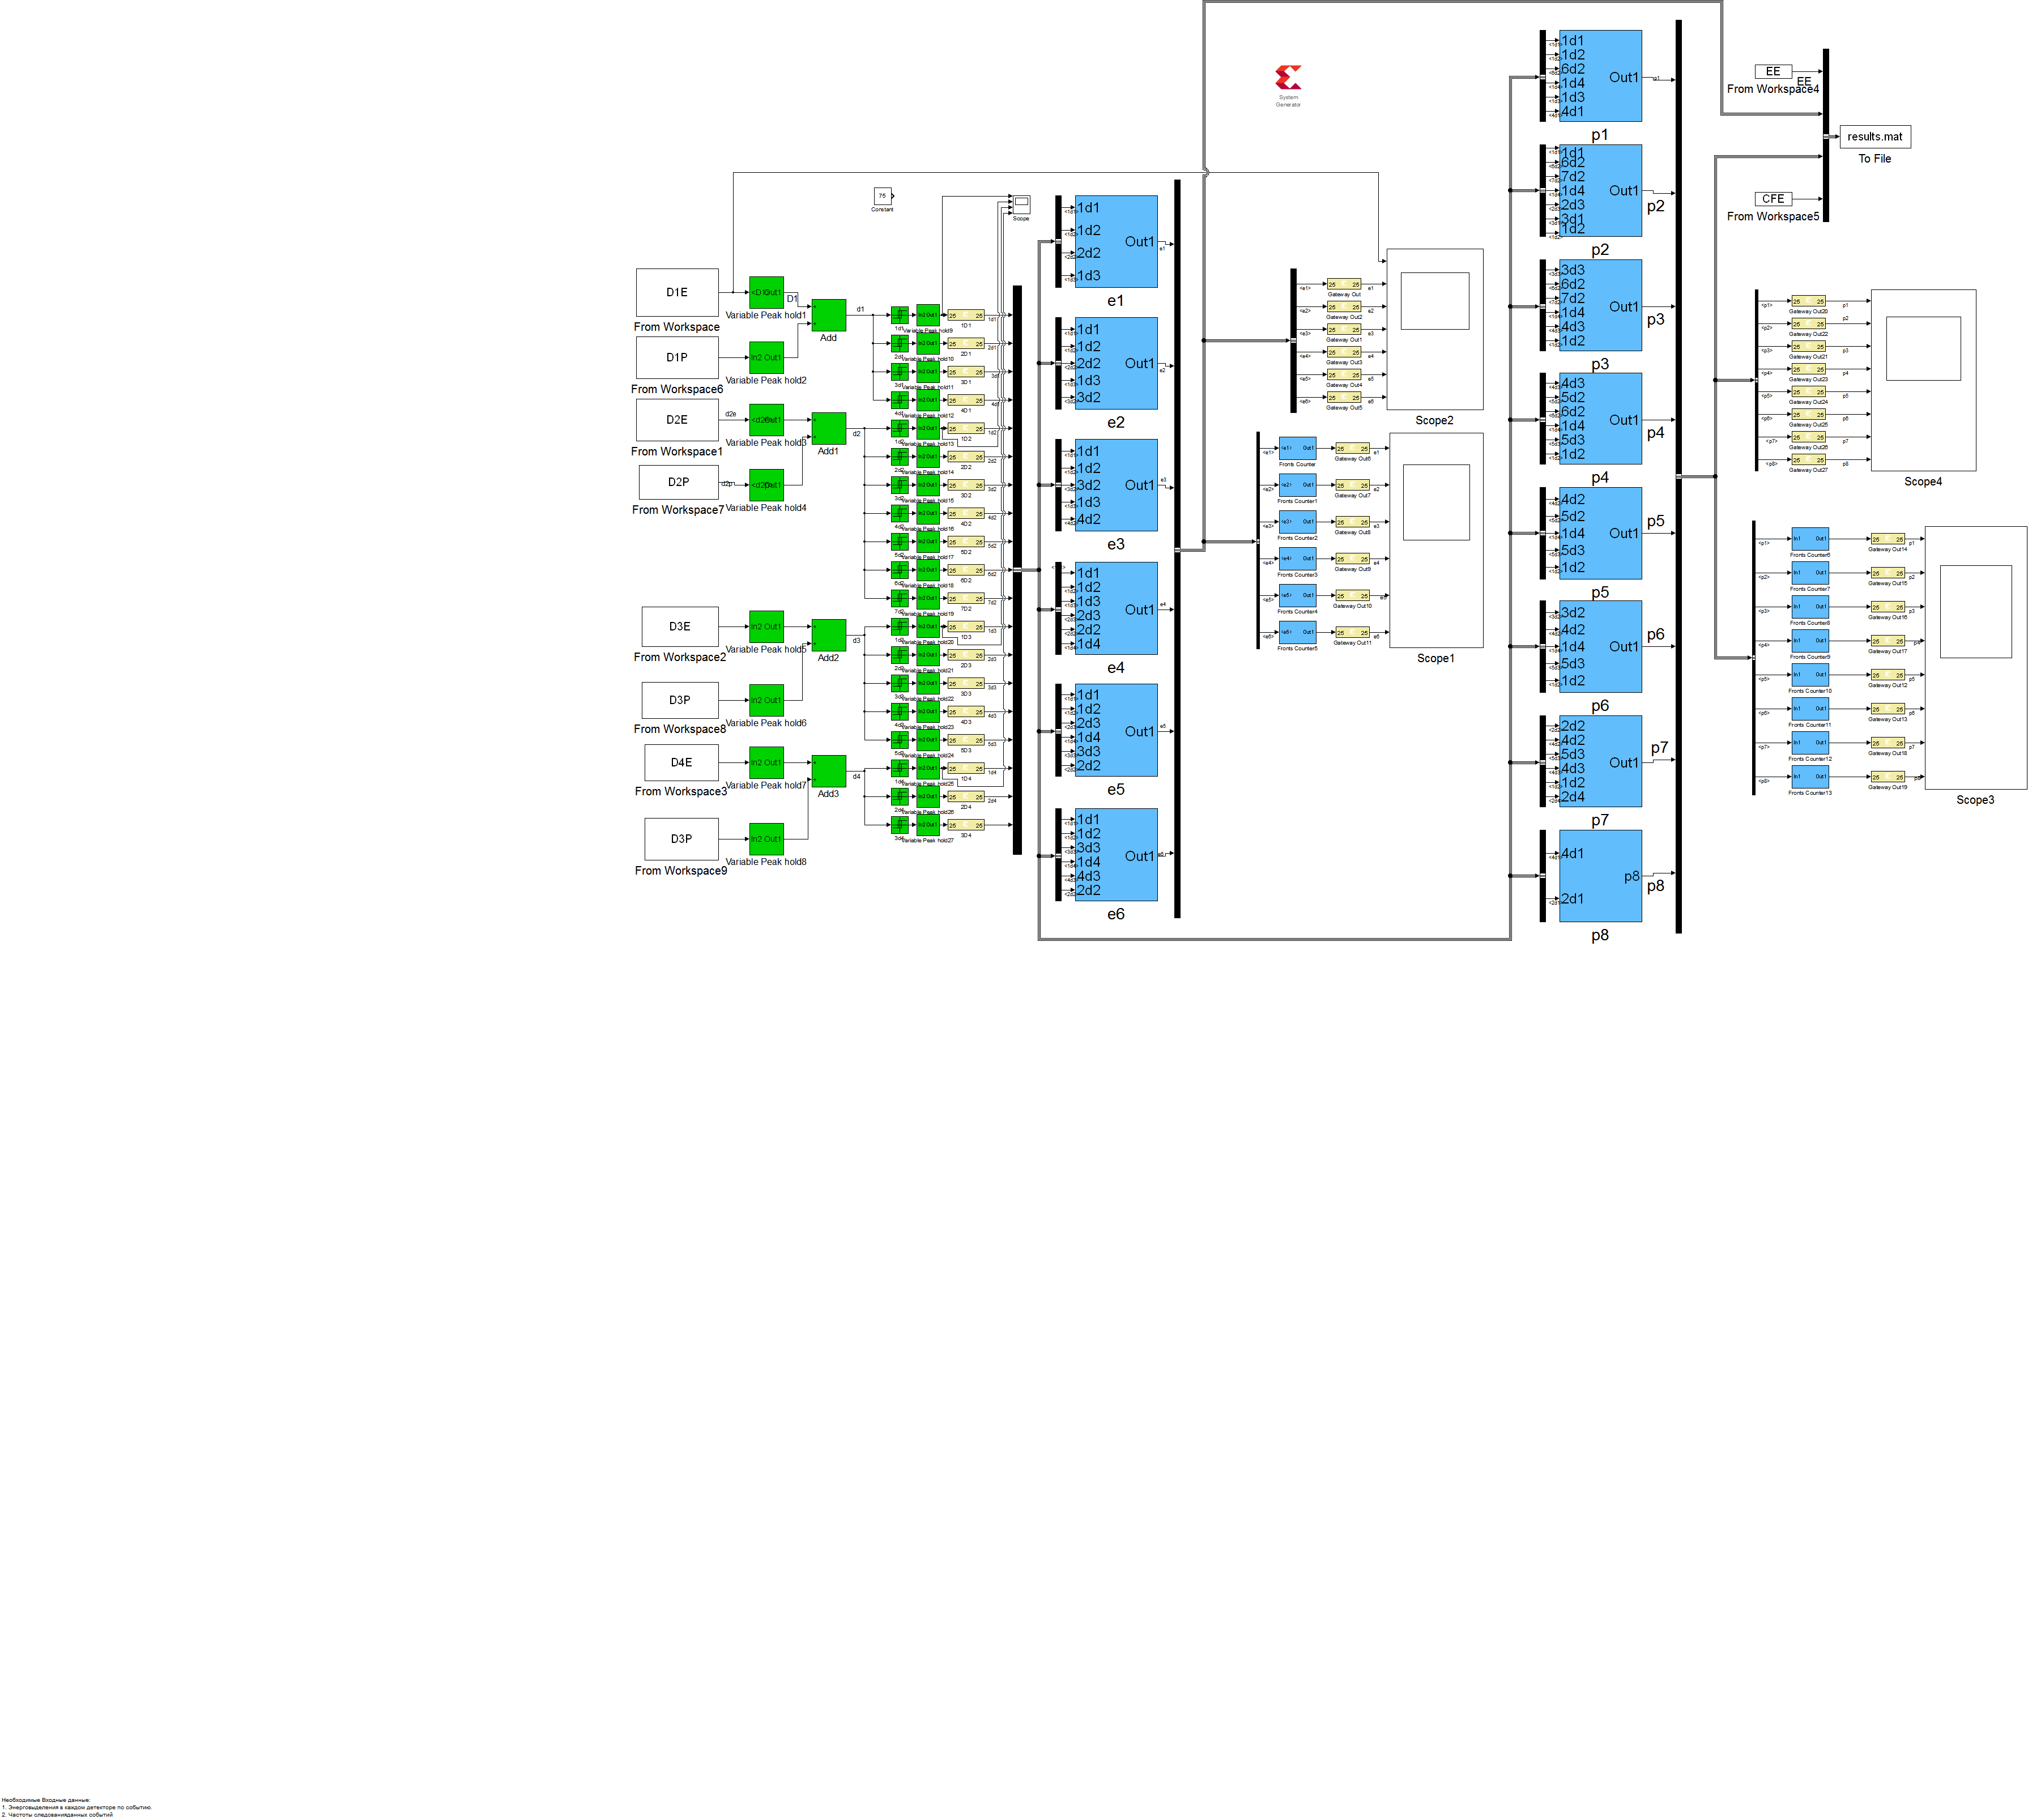
\includegraphics[width=0.7\linewidth]{images/simulink}
%	\caption{Общий вид модели прибора СПЭ в среде Simulink/Matlab. Логика определения типа и энергии частиц сгруппирована в подсистемы: е1-е6 структурные схемы выделения элекронов,  p1-p8 структурные схемы выделения протонов. D1…4E – промоделированные массивы энерговыделений в детекторах от электронов, D1…4P -  промоделированные массивы энерговыделений в детекторах от протонов. Блоки scope1-scope4 – виртуальные осциллографы в среде MATLAB, обеспечивающие наглядное отображение реакции исследуемого устройства на задаваемые внешние сигналы. Зеленым цветом показаны подсистемы имитации аналоговых сигналов, голубым цветом – подсистемы предназначенные для трансляции в аппаратный код ПЛИС, желтым цветом – выводы ПЛИС.}
%	\label{fig:simulink}
%\end{figure}

\chapter{Листингов программного кода комплекса ДЭПРОН} \label{AppendixB}


По причине проблем с поддержкой кириллицы (она встречается в комментариях и
печатаемых сообщениях), комментарии не отображены ~\ref{list:datecor}.
%\renewcommand\FBbskip{-20pt} % если хотим притянуть что-то к плавающему окружению из floatrow

\begin{ListingEnv}[H]
	% элементы, которые нежелательно разрывать обычно не ставят
	% посреди страницы: вместо H используется t (top, сверху страницы),
	% или b (bottom) или p (page, на отдельной странице)
	%    \captionsetup{format=tablenocaption}% должен стоять до самого caption
	%    \thisfloatsetup{\capposition=top}%
	\caption{Алгоритм коррекции даты в начале нового месяца на языке R}
	% далее метка для ссылки:
	\label{list:datecor}
	\begin{lstlisting}[language={Renhanced}]
	# date correction---------------------------------------------------------
	
	data.sec<-separate(data.sec, 'YYYY-MM-DD hh:mm:ss-1s',c("date", "time"),
	sep=' ')
	data.sec<-separate(data.sec, 'date',c("year", "month", "day"),
	sep='-', convert = TRUE)
	# изготовление даты из года и месяца, первого дня месяца и 12:00 по умолчанию
	data.sec$dates <- ISOdate(data.sec$year, data.sec$month, 1)
	# получение правильного дня из дня который вышел за границы месяца
	data.sec$dates <- data.sec$dates + (as.integer(data.sec$day) - 1) * 60*60*24
	# установка 00:00  
	data.sec$dates <- data.sec$dates - 60*60*12 
	# установка вермени по часам прибора
	data.sec$dates <- data.sec$dates + parse_time(data.sec$time)
	
	\end{lstlisting}
\end{ListingEnv}

%\lstset{% general command to set parameter(s)
%	basicstyle=\footnotesize} % print whole listing small
\begin{ListingEnv}
	\caption{Алгоритм коррекции ухода приборных часов на R}
	\label{list:timecor}
	\begin{lstlisting}[language={Renhanced}]
	# time correction ---------------------------------------------------------------
	
	data.sec <- data.sec%>%
	mutate(dates.UTC = data.sec$dates  - 60*60*3 )
	
	data.sec <- data.sec[,(-17:-22)]
	# data.sec$dates <- data.sec$dates - 60*60*3
	# 
	# data.sec <- data.sec%>%
	#   mutate(dates.correct.benghin =  data.sec$`YYYY-MM-DD hh:mm:ss-1s` - ceiling(
	#     56.77315002 * (data.sec$`YYYY-MM-DD hh:mm:ss-1s` - as.POSIXct('2016-08-21 09:07:00'))/86400   + 60*60*3
	#   ))
	
	# константа постоянного ухода часов прибора
	kt = (56.77315002) /86400
	# kt=  (60) /86400
	# вычитание постоянного ухода часов прибора
	# data.sec <- data.sec %>%
	#   mutate(dates.correct.benghin =  data.sec$dates.UTC - ceiling(
	#     kt* (data.sec$dates.UTC - as.POSIXct('2016-05-10 19:17:00', 'GMT'))
	#   ))
	
	data.sec <- data.sec %>%
	mutate(dates.correct.benghin =  dates.UTC - ceiling(
	kt* (dates.UTC - min(dates.UTC))
	))
	
	
	# восстановление времени начала записи в файл
	data.sec$timestamp.start <-gsub("depron-","0x",data.sec$filename)
	data.sec$timestamp.start <-gsub(".dat","",data.sec$timestamp.start)
	data.sec$timestamp.start <- as.POSIXct(as.integer(data.sec$timestamp.start), 
	origin="1970-01-01", 'GMT' )
	# data.sec$timestamp.start <- data.sec$timestamp.start -60*60*3
	
	# восстановление времни последней записи в файл
	data.sec$timestamp.end <- as.POSIXct(strptime(data.sec$timestamp,format="%d.%m.%Y %H:%M"))
	
	
	# получени разности между началом файла и горизонтальным приборным временем
	data.sec$time.delta.file.start <- as.numeric(data.sec$dates.correct.benghin - data.sec$timestamp.start ,
	units = "secs") 
	
	
	data.sec <- data.sec %>%
	group_by(filename) %>%
	distinct(filename) %>%
	summarise(delta.minimum = min(time.delta.file.start)) %>%
	left_join(data.sec, ., by = 'filename')
	
	# table(data.sec$delta.minimum)
	data.sec$time.correct.zolotarev <- data.sec$dates.correct.benghin - data.sec$delta.minimum 
	
	
	
	# отбор перескоков времени в приборе более 120 с - меньшие значения возможны при нормальной работе, 
	# большие только при отключениях питания
	data.sec <-mutate(data.sec, lag.delta = delta.minimum - lag(delta.minimum))
	table(data.sec$lag.delta)
	data.sec.switches <-filter(data.sec, abs(lag.delta) >120)
	
	
	
	data.sec <-  data.sec %>%
	mutate(switches = cut(data.sec$dates.UTC, 
	breaks = c(min(data.sec$dates.UTC),
	data.sec.switches$dates.UTC,
	max(data.sec$dates.UTC) )))
	
	# xy1 <- xyplot( delta.minimum + switches ~ timestamp.start , data = data.sec,
	#                type = c("o","g"))
	# plot(xy1)
	
	
	# plot(table(data.sec$delta.minimum))
	# table(data.sec$delta.minimum)
	# median(data.sec$delta.minimum)
	# mfv(data.sec$delta.minimum)
	
	
	
	# 
	# if(nrow(data.sec.switches)>0){
	# data.sec <-  data.sec %>%
	#   group_by(switches)  %>%
	#   mutate(med.delta =median(delta.minimum))
	# }
	# if(nrow(data.sec.switches)== 0){
	# data.sec <-  data.sec %>%
	#   mutate(med.delta =median(delta.minimum))
	# }
	
	# 
	library('modeest')
	if(nrow(data.sec.switches)>0){
	data.sec <-  data.sec %>%
	group_by(switches)  %>%
	mutate(mfv.delta =max(mfv(delta.minimum)))
	}
	if(nrow(data.sec.switches)== 0){
	data.sec <-  data.sec %>%
	mutate(mfv.delta =max(mfv(delta.minimum)))
	}
	
	
	data.sec <-  data.sec %>%
	mutate(dates.correct = dates.correct.benghin - mfv.delta)
	
	# минус минута так как данные приходят по окончании минуты
	data.sec$dates.correct <- as.POSIXct(data.sec$dates.correct, 'GMT') - 59
	
	data.sec$dates.correct.copy <- as.POSIXct(data.sec$dates.correct, 'GMT')
	# последняя проверка
	# получениЕ разности между началом файла и правильным временем
	data.sec$correct.time.delta.file.start <- as.numeric(data.sec$dates.correct - data.sec$timestamp.start ,
	units = "secs")
	\end{lstlisting}
\end{ListingEnv}

\begin{lstlisting}[language={Renhanced}]
# time correction ---------------------------------------------------------------

data.sec <- data.sec%>%
mutate(dates.UTC = data.sec$dates  - 60*60*3 )

data.sec <- data.sec[,(-17:-22)]
# data.sec$dates <- data.sec$dates - 60*60*3
# 
# data.sec <- data.sec%>%
#   mutate(dates.correct.benghin =  data.sec$`YYYY-MM-DD hh:mm:ss-1s` - ceiling(
#     56.77315002 * (data.sec$`YYYY-MM-DD hh:mm:ss-1s` - as.POSIXct('2016-08-21 09:07:00'))/86400   + 60*60*3
#   ))

# константа постоянного ухода часов прибора
kt = (56.77315002) /86400
# kt=  (60) /86400
# вычитание постоянного ухода часов прибора
# data.sec <- data.sec %>%
#   mutate(dates.correct.benghin =  data.sec$dates.UTC - ceiling(
#     kt* (data.sec$dates.UTC - as.POSIXct('2016-05-10 19:17:00', 'GMT'))
#   ))

data.sec <- data.sec %>%
mutate(dates.correct.benghin =  dates.UTC - ceiling(
kt* (dates.UTC - min(dates.UTC))
))


# восстановление времени начала записи в файл
data.sec$timestamp.start <-gsub("depron-","0x",data.sec$filename)
data.sec$timestamp.start <-gsub(".dat","",data.sec$timestamp.start)
data.sec$timestamp.start <- as.POSIXct(as.integer(data.sec$timestamp.start), 
origin="1970-01-01", 'GMT' )
# data.sec$timestamp.start <- data.sec$timestamp.start -60*60*3

# восстановление времни последней записи в файл
data.sec$timestamp.end <- as.POSIXct(strptime(data.sec$timestamp,format="%d.%m.%Y %H:%M"))


# получени разности между началом файла и горизонтальным приборным временем
data.sec$time.delta.file.start <- as.numeric(data.sec$dates.correct.benghin - data.sec$timestamp.start ,
units = "secs") 


data.sec <- data.sec %>%
group_by(filename) %>%
distinct(filename) %>%
summarise(delta.minimum = min(time.delta.file.start)) %>%
left_join(data.sec, ., by = 'filename')

# table(data.sec$delta.minimum)
data.sec$time.correct.zolotarev <- data.sec$dates.correct.benghin - data.sec$delta.minimum 



# отбор перескоков времени в приборе более 120 с - меньшие значения возможны при нормальной работе, 
# большие только при отключениях питания
data.sec <-mutate(data.sec, lag.delta = delta.minimum - lag(delta.minimum))
table(data.sec$lag.delta)
data.sec.switches <-filter(data.sec, abs(lag.delta) >120)



data.sec <-  data.sec %>%
mutate(switches = cut(data.sec$dates.UTC, 
breaks = c(min(data.sec$dates.UTC),
data.sec.switches$dates.UTC,
max(data.sec$dates.UTC) )))

# xy1 <- xyplot( delta.minimum + switches ~ timestamp.start , data = data.sec,
#                type = c("o","g"))
# plot(xy1)


# plot(table(data.sec$delta.minimum))
# table(data.sec$delta.minimum)
# median(data.sec$delta.minimum)
# mfv(data.sec$delta.minimum)



# 
# if(nrow(data.sec.switches)>0){
# data.sec <-  data.sec %>%
#   group_by(switches)  %>%
#   mutate(med.delta =median(delta.minimum))
# }
# if(nrow(data.sec.switches)== 0){
# data.sec <-  data.sec %>%
#   mutate(med.delta =median(delta.minimum))
# }

# 
library('modeest')
if(nrow(data.sec.switches)>0){
data.sec <-  data.sec %>%
group_by(switches)  %>%
mutate(mfv.delta =max(mfv(delta.minimum)))
}
if(nrow(data.sec.switches)== 0){
data.sec <-  data.sec %>%
mutate(mfv.delta =max(mfv(delta.minimum)))
}


data.sec <-  data.sec %>%
mutate(dates.correct = dates.correct.benghin - mfv.delta)

# минус минута так как данные приходят по окончании минуты
data.sec$dates.correct <- as.POSIXct(data.sec$dates.correct, 'GMT') - 59

data.sec$dates.correct.copy <- as.POSIXct(data.sec$dates.correct, 'GMT')
# последняя проверка
# получениЕ разности между началом файла и правильным временем
data.sec$correct.time.delta.file.start <- as.numeric(data.sec$dates.correct - data.sec$timestamp.start ,
units = "secs")
\end{lstlisting}
%
%Листинг~\ref{list:external1} подгружается из внешнего файла. Приходится загружать без окружения дополнительного. Иначе по страницам не переносится.
%    \lstinputlisting[lastline=78,language={R},caption={Листинг из внешнего файла},label={list:external1}]{./listings/run_analysis.R}





\begin{comment}

\chapter{Очень длинное название второго приложения, в котором продемонстрирована работа с длинными таблицами} \label{AppendixD}

 \section{Подраздел приложения}\label{AppendixB1}
Вот размещается длинная таблица:
\fontsize{10pt}{10pt}\selectfont
\begin{longtable}[c]{|l|c|l|l|}
% \caption{Описание входных файлов модели}\label{Namelists} 
%\\ 
 \hline
 %\multicolumn{4}{|c|}{\textbf{Файл puma\_namelist}}        \\ \hline
 Параметр & Умолч. & Тип & Описание               \\ \hline
                                              \endfirsthead   \hline
 \multicolumn{4}{|c|}{\small\slshape (продолжение)}        \\ \hline
 Параметр & Умолч. & Тип & Описание               \\ \hline
                                              \endhead        \hline
 \multicolumn{4}{|r|}{\small\slshape продолжение следует}  \\ \hline
                                              \endfoot        \hline
                                              \endlastfoot
 \multicolumn{4}{|l|}{\&INP}        \\ \hline 
 kick & 1 & int & 0: инициализация без шума ($p_s = const$) \\
      &   &     & 1: генерация белого шума                  \\
      &   &     & 2: генерация белого шума симметрично относительно \\
  & & & экватора    \\
 mars & 0 & int & 1: инициализация модели для планеты Марс     \\
 kick & 1 & int & 0: инициализация без шума ($p_s = const$) \\
      &   &     & 1: генерация белого шума                  \\
      &   &     & 2: генерация белого шума симметрично относительно \\
  & & & экватора    \\
 mars & 0 & int & 1: инициализация модели для планеты Марс     \\
kick & 1 & int & 0: инициализация без шума ($p_s = const$) \\
      &   &     & 1: генерация белого шума                  \\
      &   &     & 2: генерация белого шума симметрично относительно \\
  & & & экватора    \\
 mars & 0 & int & 1: инициализация модели для планеты Марс     \\
kick & 1 & int & 0: инициализация без шума ($p_s = const$) \\
      &   &     & 1: генерация белого шума                  \\
      &   &     & 2: генерация белого шума симметрично относительно \\
  & & & экватора    \\
 mars & 0 & int & 1: инициализация модели для планеты Марс     \\
kick & 1 & int & 0: инициализация без шума ($p_s = const$) \\
      &   &     & 1: генерация белого шума                  \\
      &   &     & 2: генерация белого шума симметрично относительно \\
  & & & экватора    \\
 mars & 0 & int & 1: инициализация модели для планеты Марс     \\
kick & 1 & int & 0: инициализация без шума ($p_s = const$) \\
      &   &     & 1: генерация белого шума                  \\
      &   &     & 2: генерация белого шума симметрично относительно \\
  & & & экватора    \\
 mars & 0 & int & 1: инициализация модели для планеты Марс     \\
kick & 1 & int & 0: инициализация без шума ($p_s = const$) \\
      &   &     & 1: генерация белого шума                  \\
      &   &     & 2: генерация белого шума симметрично относительно \\
  & & & экватора    \\
 mars & 0 & int & 1: инициализация модели для планеты Марс     \\
kick & 1 & int & 0: инициализация без шума ($p_s = const$) \\
      &   &     & 1: генерация белого шума                  \\
      &   &     & 2: генерация белого шума симметрично относительно \\
  & & & экватора    \\
 mars & 0 & int & 1: инициализация модели для планеты Марс     \\
kick & 1 & int & 0: инициализация без шума ($p_s = const$) \\
      &   &     & 1: генерация белого шума                  \\
      &   &     & 2: генерация белого шума симметрично относительно \\
  & & & экватора    \\
 mars & 0 & int & 1: инициализация модели для планеты Марс     \\
kick & 1 & int & 0: инициализация без шума ($p_s = const$) \\
      &   &     & 1: генерация белого шума                  \\
      &   &     & 2: генерация белого шума симметрично относительно \\
  & & & экватора    \\
 mars & 0 & int & 1: инициализация модели для планеты Марс     \\
kick & 1 & int & 0: инициализация без шума ($p_s = const$) \\
      &   &     & 1: генерация белого шума                  \\
      &   &     & 2: генерация белого шума симметрично относительно \\
  & & & экватора    \\
 mars & 0 & int & 1: инициализация модели для планеты Марс     \\
kick & 1 & int & 0: инициализация без шума ($p_s = const$) \\
      &   &     & 1: генерация белого шума                  \\
      &   &     & 2: генерация белого шума симметрично относительно \\
  & & & экватора    \\
 mars & 0 & int & 1: инициализация модели для планеты Марс     \\
kick & 1 & int & 0: инициализация без шума ($p_s = const$) \\
      &   &     & 1: генерация белого шума                  \\
      &   &     & 2: генерация белого шума симметрично относительно \\
  & & & экватора    \\
 mars & 0 & int & 1: инициализация модели для планеты Марс     \\
kick & 1 & int & 0: инициализация без шума ($p_s = const$) \\
      &   &     & 1: генерация белого шума                  \\
      &   &     & 2: генерация белого шума симметрично относительно \\
  & & & экватора    \\
 mars & 0 & int & 1: инициализация модели для планеты Марс     \\
kick & 1 & int & 0: инициализация без шума ($p_s = const$) \\
      &   &     & 1: генерация белого шума                  \\
      &   &     & 2: генерация белого шума симметрично относительно \\
  & & & экватора    \\
 mars & 0 & int & 1: инициализация модели для планеты Марс     \\
 \hline
  %& & & $\:$ \\ 
 \multicolumn{4}{|l|}{\&SURFPAR}        \\ \hline
kick & 1 & int & 0: инициализация без шума ($p_s = const$) \\
      &   &     & 1: генерация белого шума                  \\
      &   &     & 2: генерация белого шума симметрично относительно \\
  & & & экватора    \\
 mars & 0 & int & 1: инициализация модели для планеты Марс     \\
kick & 1 & int & 0: инициализация без шума ($p_s = const$) \\
      &   &     & 1: генерация белого шума                  \\
      &   &     & 2: генерация белого шума симметрично относительно \\
  & & & экватора    \\
 mars & 0 & int & 1: инициализация модели для планеты Марс     \\
kick & 1 & int & 0: инициализация без шума ($p_s = const$) \\
      &   &     & 1: генерация белого шума                  \\
      &   &     & 2: генерация белого шума симметрично относительно \\
  & & & экватора    \\
 mars & 0 & int & 1: инициализация модели для планеты Марс     \\
kick & 1 & int & 0: инициализация без шума ($p_s = const$) \\
      &   &     & 1: генерация белого шума                  \\
      &   &     & 2: генерация белого шума симметрично относительно \\
  & & & экватора    \\
 mars & 0 & int & 1: инициализация модели для планеты Марс     \\
kick & 1 & int & 0: инициализация без шума ($p_s = const$) \\
      &   &     & 1: генерация белого шума                  \\
      &   &     & 2: генерация белого шума симметрично относительно \\
  & & & экватора    \\
 mars & 0 & int & 1: инициализация модели для планеты Марс     \\
kick & 1 & int & 0: инициализация без шума ($p_s = const$) \\
      &   &     & 1: генерация белого шума                  \\
      &   &     & 2: генерация белого шума симметрично относительно \\
  & & & экватора    \\
 mars & 0 & int & 1: инициализация модели для планеты Марс     \\
kick & 1 & int & 0: инициализация без шума ($p_s = const$) \\
      &   &     & 1: генерация белого шума                  \\
      &   &     & 2: генерация белого шума симметрично относительно \\
  & & & экватора    \\
 mars & 0 & int & 1: инициализация модели для планеты Марс     \\
kick & 1 & int & 0: инициализация без шума ($p_s = const$) \\
      &   &     & 1: генерация белого шума                  \\
      &   &     & 2: генерация белого шума симметрично относительно \\
  & & & экватора    \\
 mars & 0 & int & 1: инициализация модели для планеты Марс     \\
kick & 1 & int & 0: инициализация без шума ($p_s = const$) \\
      &   &     & 1: генерация белого шума                  \\
      &   &     & 2: генерация белого шума симметрично относительно \\
  & & & экватора    \\
 mars & 0 & int & 1: инициализация модели для планеты Марс     \\ 
 \hline 
\end{longtable}

\normalsize% возвращаем шрифт к нормальному
\end{comment}

\begin{comment}
\section{Ещё один подраздел приложения} \label{AppendixB2}

Нужно больше подразделов приложения!

Пример длинной таблицы с записью продолжения по ГОСТ 2.105

    \centering
	\small
    \begin{longtable}[c]{|l|c|l|l|}
	\caption{Наименование таблицы средней длины}%
    \label{tbl:test5}% label всегда желательно идти после caption
    \\ 
    \hline
     %\multicolumn{4}{|c|}{\textbf{Файл puma\_namelist}}        \\ \hline
     Параметр & Умолч. & Тип & Описание               \\ \hline
                                                  \endfirsthead
%     \multicolumn{4}{|c|}{\small\slshape (продолжение)}        \\ \hline
 \captionsetup{format=tablenocaption,labelformat=continued}% должен стоять до самого caption
 \caption[]{} \\
    \hline
     Параметр & Умолч. & Тип & Описание               \\ \hline
                                                  \endhead        \hline
%     \multicolumn{4}{|r|}{\small\slshape продолжение следует}  \\
%\hline
                                                  \endfoot        \hline
                                                  \endlastfoot
     \multicolumn{4}{|l|}{\&INP}        \\ \hline 
     kick & 1 & int & 0: инициализация без шума ($p_s = const$) \\
          &   &     & 1: генерация белого шума                  \\
          &   &     & 2: генерация белого шума симметрично относительно \\
      & & & экватора    \\
     mars & 0 & int & 1: инициализация модели для планеты Марс     \\
     kick & 1 & int & 0: инициализация без шума ($p_s = const$) \\
          &   &     & 1: генерация белого шума                  \\
          &   &     & 2: генерация белого шума симметрично относительно \\
      & & & экватора    \\
     mars & 0 & int & 1: инициализация модели для планеты Марс     \\
    kick & 1 & int & 0: инициализация без шума ($p_s = const$) \\
          &   &     & 1: генерация белого шума                  \\
          &   &     & 2: генерация белого шума симметрично относительно \\
      & & & экватора    \\
     mars & 0 & int & 1: инициализация модели для планеты Марс     \\
    kick & 1 & int & 0: инициализация без шума ($p_s = const$) \\
          &   &     & 1: генерация белого шума                  \\
          &   &     & 2: генерация белого шума симметрично относительно \\
      & & & экватора    \\
     mars & 0 & int & 1: инициализация модели для планеты Марс     \\
    kick & 1 & int & 0: инициализация без шума ($p_s = const$) \\
          &   &     & 1: генерация белого шума                  \\
          &   &     & 2: генерация белого шума симметрично относительно \\
      & & & экватора    \\
     mars & 0 & int & 1: инициализация модели для планеты Марс     \\
    kick & 1 & int & 0: инициализация без шума ($p_s = const$) \\
          &   &     & 1: генерация белого шума                  \\
          &   &     & 2: генерация белого шума симметрично относительно \\
      & & & экватора    \\
     mars & 0 & int & 1: инициализация модели для планеты Марс     \\
    kick & 1 & int & 0: инициализация без шума ($p_s = const$) \\
          &   &     & 1: генерация белого шума                  \\
          &   &     & 2: генерация белого шума симметрично относительно \\
      & & & экватора    \\
     mars & 0 & int & 1: инициализация модели для планеты Марс     \\
    kick & 1 & int & 0: инициализация без шума ($p_s = const$) \\
          &   &     & 1: генерация белого шума                  \\
          &   &     & 2: генерация белого шума симметрично относительно \\
      & & & экватора    \\
     mars & 0 & int & 1: инициализация модели для планеты Марс     \\
    kick & 1 & int & 0: инициализация без шума ($p_s = const$) \\
          &   &     & 1: генерация белого шума                  \\
          &   &     & 2: генерация белого шума симметрично относительно \\
      & & & экватора    \\
     mars & 0 & int & 1: инициализация модели для планеты Марс     \\
    kick & 1 & int & 0: инициализация без шума ($p_s = const$) \\
          &   &     & 1: генерация белого шума                  \\
          &   &     & 2: генерация белого шума симметрично относительно \\
      & & & экватора    \\
     mars & 0 & int & 1: инициализация модели для планеты Марс     \\
    kick & 1 & int & 0: инициализация без шума ($p_s = const$) \\
          &   &     & 1: генерация белого шума                  \\
          &   &     & 2: генерация белого шума симметрично относительно \\
      & & & экватора    \\
     mars & 0 & int & 1: инициализация модели для планеты Марс     \\
    kick & 1 & int & 0: инициализация без шума ($p_s = const$) \\
          &   &     & 1: генерация белого шума                  \\
          &   &     & 2: генерация белого шума симметрично относительно \\
      & & & экватора    \\
     mars & 0 & int & 1: инициализация модели для планеты Марс     \\
    kick & 1 & int & 0: инициализация без шума ($p_s = const$) \\
          &   &     & 1: генерация белого шума                  \\
          &   &     & 2: генерация белого шума симметрично относительно \\
      & & & экватора    \\
     mars & 0 & int & 1: инициализация модели для планеты Марс     \\
    kick & 1 & int & 0: инициализация без шума ($p_s = const$) \\
          &   &     & 1: генерация белого шума                  \\
          &   &     & 2: генерация белого шума симметрично относительно \\
      & & & экватора    \\
     mars & 0 & int & 1: инициализация модели для планеты Марс     \\
    kick & 1 & int & 0: инициализация без шума ($p_s = const$) \\
          &   &     & 1: генерация белого шума                  \\
          &   &     & 2: генерация белого шума симметрично относительно \\
      & & & экватора    \\
     mars & 0 & int & 1: инициализация модели для планеты Марс     \\
     \hline
      %& & & $\:$ \\ 
     \multicolumn{4}{|l|}{\&SURFPAR}        \\ \hline
    kick & 1 & int & 0: инициализация без шума ($p_s = const$) \\
          &   &     & 1: генерация белого шума                  \\
          &   &     & 2: генерация белого шума симметрично относительно \\
      & & & экватора    \\
     mars & 0 & int & 1: инициализация модели для планеты Марс     \\
    kick & 1 & int & 0: инициализация без шума ($p_s = const$) \\
          &   &     & 1: генерация белого шума                  \\
          &   &     & 2: генерация белого шума симметрично относительно \\
      & & & экватора    \\
     mars & 0 & int & 1: инициализация модели для планеты Марс     \\
    kick & 1 & int & 0: инициализация без шума ($p_s = const$) \\
          &   &     & 1: генерация белого шума                  \\
          &   &     & 2: генерация белого шума симметрично относительно \\
      & & & экватора    \\
     mars & 0 & int & 1: инициализация модели для планеты Марс     \\
    kick & 1 & int & 0: инициализация без шума ($p_s = const$) \\
          &   &     & 1: генерация белого шума                  \\
          &   &     & 2: генерация белого шума симметрично относительно \\
      & & & экватора    \\
     mars & 0 & int & 1: инициализация модели для планеты Марс     \\
    kick & 1 & int & 0: инициализация без шума ($p_s = const$) \\
          &   &     & 1: генерация белого шума                  \\
          &   &     & 2: генерация белого шума симметрично относительно \\
      & & & экватора    \\
     mars & 0 & int & 1: инициализация модели для планеты Марс     \\
    kick & 1 & int & 0: инициализация без шума ($p_s = const$) \\
          &   &     & 1: генерация белого шума                  \\
          &   &     & 2: генерация белого шума симметрично относительно \\
      & & & экватора    \\
     mars & 0 & int & 1: инициализация модели для планеты Марс     \\
    kick & 1 & int & 0: инициализация без шума ($p_s = const$) \\
          &   &     & 1: генерация белого шума                  \\
          &   &     & 2: генерация белого шума симметрично относительно \\
      & & & экватора    \\
     mars & 0 & int & 1: инициализация модели для планеты Марс     \\
    kick & 1 & int & 0: инициализация без шума ($p_s = const$) \\
          &   &     & 1: генерация белого шума                  \\
          &   &     & 2: генерация белого шума симметрично относительно \\
      & & & экватора    \\
     mars & 0 & int & 1: инициализация модели для планеты Марс     \\
    kick & 1 & int & 0: инициализация без шума ($p_s = const$) \\
          &   &     & 1: генерация белого шума                  \\
          &   &     & 2: генерация белого шума симметрично относительно \\
      & & & экватора    \\
     mars & 0 & int & 1: инициализация модели для планеты Марс     \\ 
     \hline 
    \end{longtable}
\normalsize% возвращаем шрифт к нормальному
\end{comment}